\appendix
\chapter{MS-DOS Virussen}

Een belangrijke functie van het besturingssysteem is het beveiligen van het systeem. Met de geconnecteerde wereld die we vandaag kennen, is dit misschien zelfs \'e\'en van de hoofdtaken geworden van het besturingssysteem. Dat is echter niet altijd zo geweest: zoals besproken in Hoofdstuk~\ref{hfdstk:inleiding} is een besturingssysteem origineel ontstaan als een programma om het beheer van processen te vereenvoudigen. Ook het eerste besturingssysteem van Microsoft, het \emph{Microsoft Disk Operating System (MS-DOS)} diende vooral om het procesbeheer te vergemakkelijken en het aansturen van bepaalde hardware (zoals bijvoorbeeld de harde schijf) te vereenvoudigen. Het bood echter geen bescherming. Zo draaide elk proces bijvoorbeeld in kernel mode, waardoor het dus toegang had tot de volledige instructieset die de processor aanbood. Hierdoor kunnen processen rechtstreeks communiceren met hardware en zijn ze dus niet verplicht om via de MS-DOS-aangeleverde routines de hardware te benaderen.

Over het algemeen werkte dit principe goed. Er kon slechts \'e\'en proces tegelijkertijd actief zijn (MS-DOS ondersteunde dus geen multi-programmering), dus kan het actieve proces ook nooit in het vaarwater komen van andere processen aangezien die er niet zijn. De meeste programma's maakten ook gebruik van de services die MS-DOS aanbood om bijvoorbeeld bestanden te openen of uitvoer op het scherm te tonen.

Omdat programma's echter niet gecontroleerd werden door het besturingssysteem, is het niet te verwonderen dat er ook heel wat \emph{malware} gebouwd is geweest voor MS-DOS. Dat nam typische de vorm aan van een virus dat het systeem infecteerde en op bepaalde tijdstippen de correcte werking van het systeem verstoorde. In dit hoofdstuk bespreken we enkele voorbeelden, en leggen we uit waarom deze virussen niet meer kunnen werken in hedendaagse besturingssystemen.

\section{Virussen}

De term \emph{virus} wordt door leken vaak gebruikt voor eender welk stuk software dat een ongewenste en/of kwaadaardige nevenwerking heeft op een computer. Dat is natuurlijk niet correct: een betere term hiervoor is \emph{malware} (wat komt van \emph{malicious software}, of kwaadaardige software). Een virus is een heel specifieke categorie van malware die vroeger veel voorkwam, maar vandaag de dag minder relevant is. De definitie van een virus die wij gebruiken, luidt als volgt:

\begin{quotation}
Een computervirus is een type van kwaadaardige software dat, wanneer het uitgevoerd wordt, zichzelf vermenigvuldigt door aan andere (onschuldige) computerprogramma's een kopie van zichzelf toe te voegen.
\end{quotation}

Cruciaal aan deze definitie is dat een virus dus een bestaand programma aanpast; het bestaat niet op zichzelf. Dit gedrag was belangrijk, want de manier waarop virussen zich vroeger verspreidden was door onschuldige software te infecteren die dan via diskette's onderling tussen mensen werd uitgewisseld. In die tijd wisten computergebruikers precies welk programmabestand overeenkwam met bijvoorbeeld de tekstverwerker die ze gebruikten. Onbekende programma's vielen dus direct op, en zouden niet snel opgestart worden.

Vandaag de dag zijn er veel makkelijkere manieren om malware op een computer te krijgen. De eenvoudige aanpak van de \emph{Happy '99}-worm illustreert dit punt. Rond nieuwjaar 1999 kregen heel wat mensen een email met als onderwerp `Happy 99' die verder leeg was op een bijlage na. Deze bijlage was een uitvoerbaar bestand `Happy99.exe'. Wanneer dit bestand opgestart werd, kreeg de gebruiker vuurwerk te zien (zie Figuur~\ref{happy99}), maar in de achtergrond werd ook het adressenboek doorgenomen en werd de worm doorgestuurd naar elk emailadres dat daarin gevonden werd. Het internet zorgt er voor dat malware zich in een recordtempo op een ongeziene schaal kan verspreiden. Ook gebruiken meer mensen nu een computer, wat er toe leidt dat niet iedereen even goed weet hoe een computer werkt en ook niet iedereen even strikt is in het installeren van belangrijke programma-updates.

\begin{figure}
\begin{center}
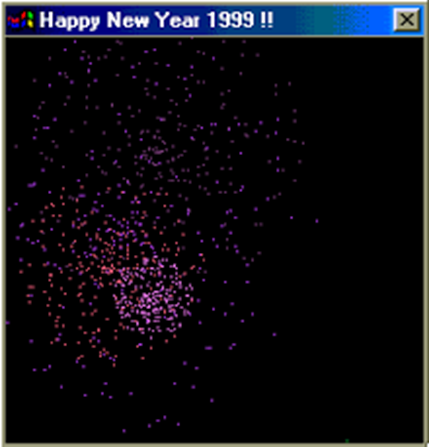
\includegraphics[width=70mm]{images/happy99.png}
\end{center}
\caption{De Happy 99-worm}
\label{happy99}
\end{figure}

Virussen voor MS-DOS waren meestal relatief goedaardig. Ze waren veelal een manier om op te scheppen over de technische kwaliteiten die de auteur van zo'n virus had. Zo toonde ze vaak gewoon een bericht op het scherm, eventueel aangevuld met een (tekstuele) tekening. Soms plaagden ze de gebruiker, bijvoorbeeld door de letters van het scherm te laten vallen of door ze te verplichten om eerst een spelletje te spelen. Er waren echter ook kwaadaardige virussen in omloop. Het Casino-virus, bijvoorbeeld, verwijderde de FAT-tabel van de harde schijf en forceerde de gebruiker om een jackpot-spel te spelen. Indien de gebruiker won (waar 17.2\% kans voor was), dan werd een geheugenkopie van de FAT terug naar de schijf gekopie\"eerd. Indien de gebruiker niet won, was hij natuurlijk al zijn bestanden kwijt. Een nog erger voorbeeld was het \emph{CMOSdead}-virus. Dit virus maakte de ROM-chip stuk waar de opstartcode van de computer in stond. Hierdoor kon de computer dus niet meer opstarten. Verder begon hij een irritant lawaai te maken, en formateerde hij de harde schijf indien de gebruiker op CTRL-ALT-DEL drukte.

Onafhankelijk van de goed- of kwaadaardigheid van een virus, staat het vast dat de auteurs bijzonder diepgaande kennis moesten hebben van MS-DOS en computers in het algemeen om zulke software te schrijven. In het bijzonder zijn dit een aantal onderwerpen die je als virusschrijver helemaal onder de knie moest hebben:

\begin{itemize}
\item{\textbf{x86 Assembly}} Virussen moesten klein zijn en gebruikten vaak processorinstructies die niet rechtstreeks bruikbaar zijn vanuit hogere programmeertalen. Daarom werden de meeste virussen ook rechtstreeks in x86 assembly geschreven.
\item{\textbf{Bootproces}} Een populaire plaats om te infecteren was de code van het bootproces. Dit houdt natuurlijk in dat je perfect moet weten wat er allemaal gebeurt wanneer je computer opstart.
\item{\textbf{Interrupts}} De meeste virussen infecteerden de interrupttabel, zodat ze automatisch opgeroepen werden wanneer bepaalde interrupt requests zich voordeden.
\item{\textbf{.EXE-formaat}} Virussen voegden zichzelf toe aan andere programma's. Kennis van het formaat van een .EXE-bestand is dus vereist.
\item{\textbf{Cryptografie/steganografie}} Voor extra bescherming tegen virusscanners kon een virus zichzelf gaan encrypteren of verstoppen.
\end{itemize}

\section{Bootsector-virussen}

Het \emph{Stoned}-virus\footnote{\url{https://en.wikipedia.org/wiki/Stoned_(computer_virus)}} was een voorbeeld van een \emph{bootsector-virus}. Deze virussen spitsen zich toe op het infecteren van de opstartcode die op de harde schijf of op een diskette staat. Het Stoned-virus toont in 12.5\% van de keren dat je je computer opstart de zin ``Your PC is now Stoned!'' of ``Legalise Marijuana''. Figuur~\ref{stoned} toont de bootsector van een harde schijf die ge\"infecteerd is met het Stoned-virus. In de rechterkolom kan je onderaan de tekst zien staan.

\begin{figure}
\begin{center}
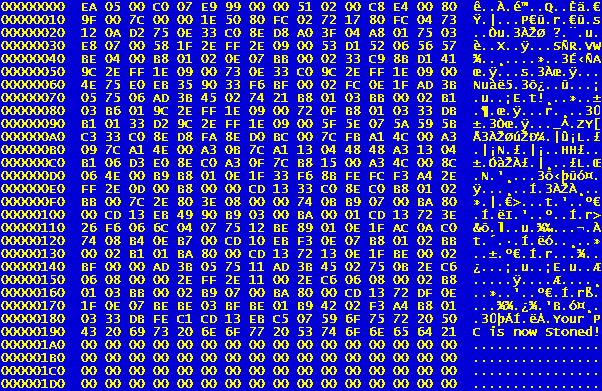
\includegraphics[width=120mm]{images/stoned.png}
\end{center}
\caption{De bootsector van een ge\"infecteerde computer.}
\label{stoned}
\end{figure}

In Hoofdstuk~\ref{bootproces} hebben we gezien dat moderne computers opstarten volgens de stappen die in de UEFI-standaard vastgelegd zijn. DOS is echter gemaakt voor computers die de voorloper van UEFI gebruikten: het \emph{Basic Input/Output System (BIOS)}. De BIOS is in feite een mini-programma dat de computer initialiseert en op zoek gaat naar een opstartmedium. Als er moet opgestart worden van de harde schijf, dan gaat de BIOS de eerste sector van die schijf (de \emph{Master Boot Record}) in het geheugen laden. De BIOS springt dan naar een miniprogramma dat in de MBR staat (de \emph{Initial Program Loader}, of \emph{IPL}). De IPL zoekt dan tussen de partities van de schijf naar de actieve partitie (d.i. de partitie waar het op te starten besturingssysteem op staat). Wanneer die partitie gevonden is, wordt de eerste sector van die partitie (de \emph{boot sector}) in het geheugen gezet, en springt de IPL naar een mini-programma dat in deze boot sector staat (de \emph{boot loader}). De boot loader is besturingssysteem-afhankelijk en heeft de taak om het besturingssysteem verder op te starten. Figuur~\ref{boot-sequence} toont dit proces schematisch.

\begin{figure}
\begin{center}
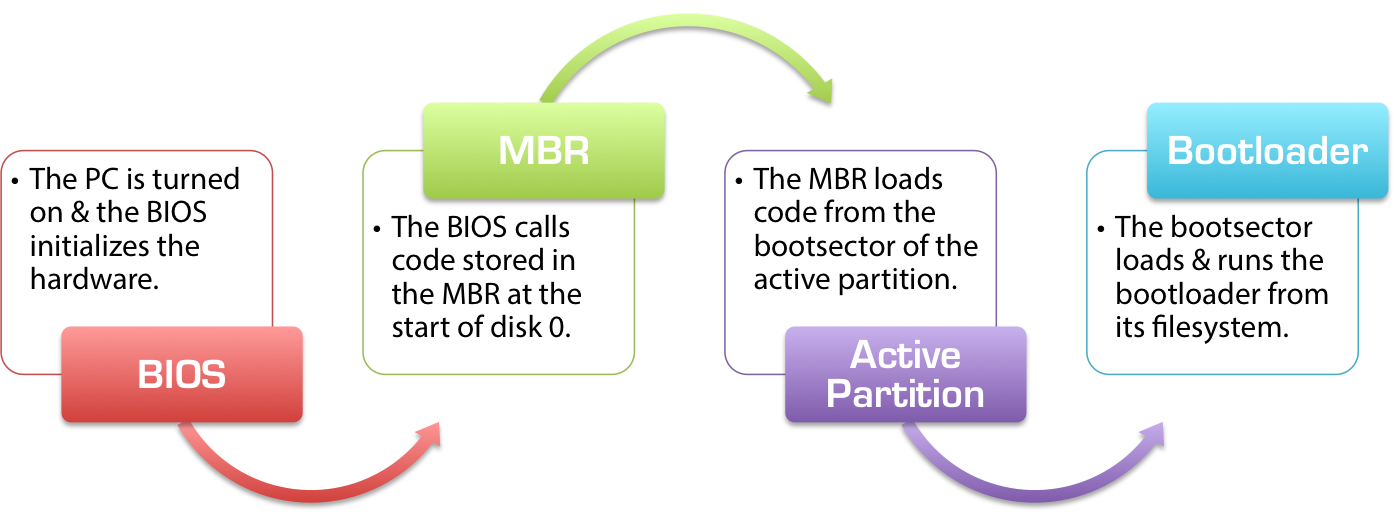
\includegraphics[width=125mm]{images/MBR-Boot-Sequence.png}
\end{center}
\caption{Het opstartproces van een computer met BIOS firmware.}
\label{boot-sequence}
\end{figure}

Stel dat de computer een diskette bevat die ge\"infecteerd is met het Stoned-virus. De BIOS controleert tijdens het opstarten of er een diskette in de computer steekt, en als dat het geval is (en als de diskette \emph{bootable} is) gaat hij daarvan opstarten. Dit wil zeggen dat de eerste sector van de diskette naar het geheugen wordt gekopi\"eerd en dat de BIOS springt naar het programma dat hierin vervat zit. Aangezien het om een ge\"infecteerde diskette gaat, is dit programma dus het Stoned-virus dat uitgevoerd wordt. Het eerste wat Stoned doet, is de harde schijf infecteren. De originele master boot record wordt ergens anders op de schijf opgeslagen, en het virus wordt gekopie\"erd. Verder wordt ook interrupt 13h onderschept door eenvoudigweg de interrupttabel aan te passen zodat die naar een methode van het virus wijst. Interrupt 13h wordt door DOS gebruikt voor lees- of schrijfoperaties van sectoren. Het resultaat is dat elke lees- of schrijfoperatie die uitgevoerd wordt door eender welk programma het virus activeert. Wanneer het virus een onge\"infecteerde diskette detecteert, dan infecteert hij die eerst alvorens de originele interrupt-aanvraag te verwerken.

\section{Executable infectors}

Het \emph{Phantom1}-virus is een voorbeeld van een \emph{executable infector}. Deze virussen plaatsen een kopie van zichzelf in de programma's die de gebruiker uitvoert. Phantom1 wordt geactiveerd wanneer er ongeveer 20 minuten geen toetsenbordactiviteit is. Het toetsenbord wordt gedeactiveerd en de gebruiker krijgt een boodschap te zien en een geanimeerd doodshoofd (zie Figuur~\ref{phantom1}).

\begin{figure}
\begin{center}
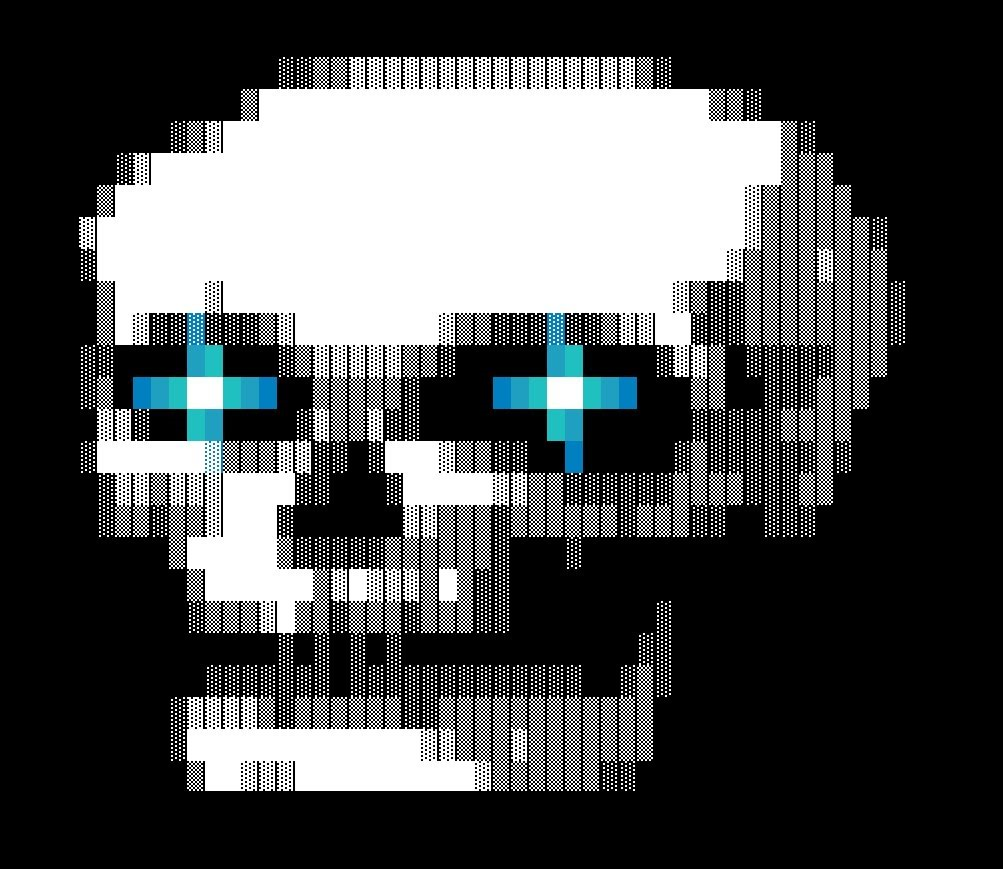
\includegraphics[width=80mm]{images/Phantom1.png}
\end{center}
\caption{Het Phantom1-virus in actie.}
\label{phantom1}
\end{figure}

Het virus kent de structuur van een uitvoerbaar bestand, en weet dat in de hoofding van een .EXE-bestand het adres staat van de instructie waarmee het programma op moet starten. Het virus kan zichzelf dus toevoegen aan het code sectie en kan dit opstartadres in de hoofding overschrijven. Wanneer het programma dan opgestart wordt, zal het eerst de code van het virus opstarten alvorens het virus terugspringt naar de normale opstartprocedure van het programma.

Phantom1 past ook de interrupttabel aan, meerbepaald de adressen voor de interrupts 1Ch en 21h. Interrupt 1Ch wordt periodiek opgeroepen door de klok van het systeem, terwijl interrupt 21h door DOS gebruikt wordt voor onder andere allerlei bestandsoperaties en het inlezen van toetsenbordinvoer. Hierdoor kan Phantom1 meten wanneer er 20 minuten geen toetsenbordactiviteit is geweest. Ook wanneer er een nieuw programma opgestart wordt, zal DOS interrupt 21h activeren. Phantom1 gaat in dit geval het programma meteen infecteren.

\section{De viruswapenwedloop}

Naarmate MS-DOS meer last begon te krijgen van virussen, werd er gezocht naar oplossingen om deze virussen te kunnen detecteren of zelfs verwijderen. Al snel na de eerste virussen kwam ook de eerste generatie van virusscanners. Om slechts een kleine impact op de snelheid van het systeem te hebben, werkten deze scanners nogal eenvoudig. Zo werd de harde schijf bijvoorbeeld een eerste keer gescanned en werd er een database bijgehouden van alle groottes van de uitvoerbare bestanden. Periodiek werd de harde schijf dan terug gescanned en werd de grootte van alle programma's vergeleken met de data van de database. Als er een programma \emph{gegroeid} was, dan was het waarschijnlijk ge\"infecteerd door een virus. Deze aanpak was natuulijk eenvoudig te omzeilen: in plaats van de code van het virus achter het originele programma te plakken, werd er gewoon een stuk van het originele programma overschreven. Mettertijd werden de virusscanners dan ook geavanceerder en gingen ze meer op zoek gaan naar bepaalde patronen die op een virusinfectie konden wijzen (bijv. een opeenvolging van bepaalde instructies). Naarmate dat virusscanners beter werden, werden ook de virussen beter. Er ontstond dus als het ware een wapenwedloop tussen de auteurs van de virussen en de auteurs van de virusscanners.

Een \emph{stealth virus} verborg de aanpassingen die het gemaakt had aan het systeem. Dit werd onder andere gedaan door de systeemfunctie om sectoren te lezen te kapen. De resultaten van deze functie werden dan vervalst, zodat het oproepend programma de infectie niet zou kunnen waarnemen.

Een \emph{polymorf virus} produceerde werkende kopie\"en van zichzelf die er allen verschillend uitzagen. Op die manier kon een virusscanner niet zoeken naar een bepaald vast patroon dat in het virus voorkwam, aangezien elke kopie van het virus er anders uitzag. Een relatief eenvoudige manier om het gewenste effect te bekomen, was door het virus zichzelf te laten encrypteren.

Een \emph{gepantserd virus} maakte gebruik van allerlei anti-debugging trucs en gebruikte code die expres moeilijk en onlogisch in elkaar zat. Dit maakte het werk van de virusanalisten moeilijker, zodat het langer duurde eer er een virusscanner was die een effectieve beveiliging vormde tegen het virus.

Ondertussen is MS-DOS vervangen door Windows, en geeft het besturingssysteem niet meer de volledige toegang tot de hardware aan eender welke applicatie. Heel wat technologie\"en die we in de vorige hoofdstukken gezien hebben zorgen er voor dat een virus vandaag niet meer zo effectief zou zijn als het ooit was. Zo bevat een modern besturingssysteem bijvoorbeeld deze tegenmaatregelen:

\begin{itemize}
\item{\textbf{UEFI Secure Boot}} Alle code die uitgevoerd wordt tijdens het opstartproces wordt cryptografisch ondertekend. Alvorens de processor de code uitvoert, wordt steeds de handtekening gecontroleerd. Mocht de originele code veranderd zijn, dan zal de handtekening niet meer kloppen en zal de UEFI-implementatie de code niet uitvoeren.
\item{\textbf{Geheugenbescherming}} Programma's worden uitgevoerd in afgeschermde stukken geheugen. Het ene programma kan dus niet zomaar een stuk geheugen aanpassen van een ander programma of van het besturingssysteem.
\item{\textbf{Bestandspermissies}} Besturingssystemen dwingen bestandspermissies af, waardoor een bestand bijvoorbeeld leesbaar kan zijn maar niet schrijfbaar. In Windows zijn bijvoorbeeld de programma's die op de standaardplek ge\"installeerd worden (c:\textbackslash{}Program Files) \emph{niet} schrijfbaar.
\item{\textbf{Codehandtekeningen}} De code in programma's kan een cryptografische handtekening krijgen. Wanneer het besturingssysteem zo'n handtekening controleert en die niet overeenstemt met de feitelijke code, dan zal het programma niet opgestart worden.
\item{\textbf{Monitoring van hardwaretoegang}} Elke toegang tot een hardwareapparaat verloopt via het besturingssysteem. Een programma kan dus niet rechtstreeks communiceren met hardware. Het besturingssysteem krijgt steeds de kans om de toegang te monitoren en eventueel te verbieden.
\item{\textbf{Geavanceerde virusscanners}} Hedendaagse virusscanners doen veel meer dan het zoeken naar bepaalde patronen in code. Wanneer het voor een virusscanner niet duidelijk is of een bepaald stuk van een programma een virus zou kunnen zijn (bijv. omdat het virus zich ge\"encrypteerd heeft), dan kan de virusscanner de verdachte code emuleren. De code wordt dan als het ware uitgevoerd onder veilige omstandigheden en geanalyseerd.
\end{itemize} 